\everymath{\displaystyle}
\documentclass{beamer}
% \documentclass[handout]{beamer}

%\usepackage[pdftex]{color,graphicx}
\usepackage{amsmath,amssymb,amsfonts}

\mode<presentation>
{
  % \usetheme{Darmstadt}
  % \usetheme[hideothersubsections]{Hannover}
  % \usetheme[hideothersubsections]{Goettingen}
  \usetheme[hideothersubsections, right]{Berkeley}

  \usecolortheme{seahorse}
  % \usecolortheme{dolphin}
  \usecolortheme{rose}
  % \usecolortheme{orchid}

  \useinnertheme[shadow]{rounded}

  \setbeamercovered{transparent}
  % or whatever (possibly just delete it)
}

\mode<handout>{
  \setbeamercolor{background canvas}{bg=black!5}
  \usepackage{pgfpages}
  \pgfpagesuselayout{4 on 1}[a4paper,border shrink=5mm, landscape]
}

\usepackage[brazilian]{babel}
% or whatever

% \usepackage[latin1]{inputenc}
\usepackage[utf8]{inputenc}
% or whatever

\usepackage{times}
%\usepackage[T1]{fontenc}
% Or whatever. Note that the encoding and the font should match. If T1
% does not look nice, try deleting the line with the fontenc.


\title%[] % (optional, use only with long paper titles)
{Comparando médias de 2 grupos}

\subtitle
{Intervalos de Confiança da diferença entre as médias} % (optional)

\author%[] % (optional, use only with lots of authors)
{Felipe Figueiredo}% \and S.~Another\inst{2}}
% - Use the \inst{?} command only if the authors have different
%   affiliation.

\institute[] % (optional, but mostly needed)
{
}
  % \inst{1}%
  % Department of Computer Science\\
  % University of Somewhere
  % \and
  % \inst{2}%
  % Department of Theoretical Philosophy\\
  % University of Elsewhere}
% - Use the \inst command only if there are several affiliations.
% - Keep it simple, no one is interested in your street address.

\date%[] % (optional)
{}

% \subject{Talks}
% This is only inserted into the PDF information catalog. Can be left
% out. 



% If you have a file called "university-logo-filename.xxx", where xxx
% is a graphic format that can be processed by latex or pdflatex,
% resp., then you can add a logo as follows:

\pgfdeclareimage[height=1.6cm]{university-logo}{../logo}
\logo{\pgfuseimage{university-logo}}



% Delete this, if you do not want the table of contents to pop up at
% the beginning of each subsection:
\AtBeginSubsection[]
%\AtBeginSection[]
{
  \begin{frame}<beamer>{Sumário}
    \tableofcontents[currentsection,currentsubsection]
  \end{frame}
}


% If you wish to uncover everything in a step-wise fashion, uncomment
% the following command: 

% \beamerdefaultoverlayspecification{<+->}


\begin{document}

\begin{frame}
  \titlepage
\end{frame}

\begin{frame}{Sumário}
  \tableofcontents
  % You might wish to add the option [pausesections]
\end{frame}


%% Template
% \section{}

% \subsection{}

% \begin{frame}{}
%   \begin{itemize}
%   \item 
%   \end{itemize}
% \end{frame}

% \begin{frame}
%   \begin{columns}
%     \begin{column}{5cm}
%     \end{column}
%     \begin{column}{5cm}
%     \end{column}
%   \end{columns}
% \end{frame}

% \begin{frame}{}
%   \includegraphics[height=0.4\textheight]{file1}
%   \includegraphics[height=0.4\textheight]{file2}
%   \includegraphics[height=0.4\textheight]{file3}
%   \begin{figure}
%     \caption{}
%   \end{figure}
% \end{frame}

% \begin{frame}{}
%   \begin{definition}
%   \end{definition}
%   \begin{example}
%   \end{example}
%   \begin{block}{Exercício}
%   \end{block}
% \end{frame}

\section[t de Student]{A distribuição t de Student}

\subsection{A distribuição t de Student}

\begin{frame}{Recapitulando}
  \begin{itemize}
  \item Vimos que o IC é composto de 3 componentes
    \begin{itemize}
    \item a média $\bar{x}$ (tendência central)
    \item o erro padrão da média (SEM)
    \item um tal de $t^{*}$, que depende de $n$
    \end{itemize}
  \item Como N era grande, utilizamos $t^{*} \approx 2$
    \bigskip
  \item Mas de onde vem esse $t^{*}$? Qual seria o valor correto?
  \end{itemize}
\end{frame}

\begin{frame}{A distribuição T de Student}
  \begin{center}
    
\includegraphics[height=\textheight]{Cap5/Guinness}
  \end{center}
\end{frame}

\begin{frame}{A distribuição T de Student}
  \begin{center}
    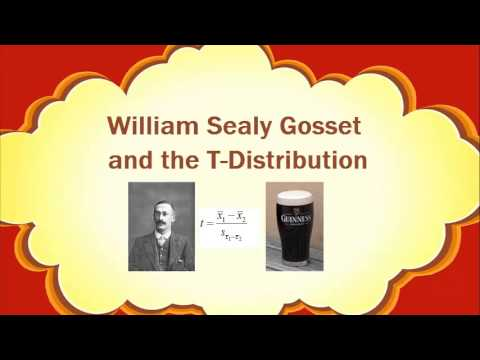
\includegraphics[height=\textheight]{Cap5/Student-Guinness}
  \end{center}
\end{frame}

\begin{frame}{A distribuição t de Student}
  \begin{itemize}
  \item Student (pseudônimo de W. S. Gossett [1876-1937], trabalhando
    para a cervejaria Guiness) criou uma distribuição que melhor se
    aproxima dos dados de amostras pequenas
%  \item É semelhante à Normal padrão, mas tem variância maior
  \item Tem um parâmetro \alert{graus de liberdade} ({\em df} em inglês) vinculado ao tamanho da amostra $n$.
    % \begin{displaymath}
    %   gl = n-1
    % \end{displaymath}
  \end{itemize}
\end{frame}

\begin{frame}{A distribuição t de Student}
  \begin{figure}
    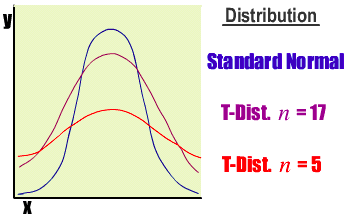
\includegraphics[height=0.7\textheight]{Inf_II/t_graph}
    \caption{A distribuição t de Student}
  \end{figure}
\end{frame}

\begin{frame}{Propriedades da distribuição t}
  \begin{itemize}
  \item A distribuição tem forma de sino (simétrica) assim como a
    Normal padrão Z
  \item Reflete a maior variabilidade inerente às amostras pequenas
  \item O formato da curva depende do tamanho da amostra $n$
  \item Quanto mais graus de liberdade (dados), mais a distribuição
    $t$ se parece com a distribuição $Z$.
  \end{itemize}
\end{frame}

% \begin{frame}{A tabela t}
%   \begin{center}
%     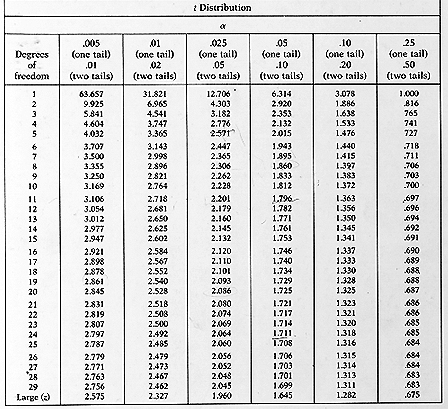
\includegraphics[height=0.9\textheight]{Inf_II/t_table}
%   \end{center}
% \end{frame}

\begin{frame}{Alguns valores de t, para diferentes graus de liberdade}
  \begin{itemize}
  \item $N = 5 \Rightarrow t = 2.776$
  \item $N = 10 \Rightarrow t = 2.262$
  \item $N = 15 \Rightarrow t = 2.145$
  \item $N = 20 \Rightarrow t = 2.093$
  \item $N = 30 \Rightarrow t = 2.045$
  \end{itemize}
  \begin{block}{}<2->
    \begin{itemize}
    \item Para N  grande, $t \rightarrow 1.960$
    \end{itemize}
  \end{block}
\end{frame}

\section[IC diferença 2 médias]{Intervalo de Confiança da diferença entre duas médias}

\subsection{Interpretaçãao}

\subsection{Participantes: pareados ou não-pareados?}

\end{document}
